% !TEX root = ../main.tex
%!TeX spellcheck = es-CL
\documentclass[../main.tex]{subfiles}

\chapter{Conceptos Básicos}

\section*{Introducción}

\NC{Insertar 'frase profunda' + 'Introducción pertinente'}

\section{Grafos}

Un \textbf{grafo} corresponde a un objeto utilizado para
modelar relaciones entre elementos de un sistema o conjunto. Su
origen y denominación, se basan en la representación de estas
relaciones por medio de esquemas gráficos caracterizados por
segmentos entre \textit{ vértices } o (nodos) y \textit{aristas}.

\begin{definition}[Grafo]
\label{def:grafo}

Dados los conjuntos $ V $ y $ E \subseteq \binom{ V }{ 2 }$
\footnote{Si $X$ es un conjunto, se denota por $\binom{ X }{ 2 }$ al
conjunto de pares (no ordenados) de la forma $\lbrace { u , v }
\rbrace$ donde $ u \neq v $ para $ u , v \in X$.}. Se define como
\textbf{grafo} al par $G = ( V , E)$. En este contexto, el conjunto $V$
se denota como el conjunto de \textbf{vértices} de $G$ y $E$ como su
conjunto de \textbf{aristas}.

\end{definition}

A modo de ejemplo, se muestra en la figura \ref{fig:1} una
representación para un grafo con $9$ vértices.

\begin{figure}[ht]
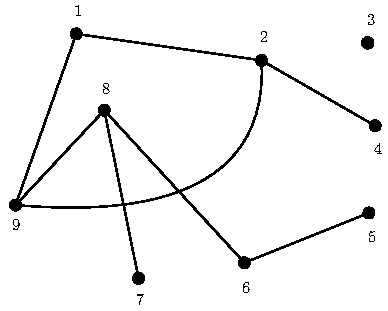
\includegraphics[scale=0.85]{./figuras/pdf/fig1.pdf}
\caption{Representación del grafo $G = (V,E)$ dado por los
	vértices $V= \lbrace {1,2,3,4,5,6,7,8,9} \rbrace$. Sus aristas
	corresponden a los segmentos que unen estos a vértices y se
	denotan con los pares $E = \lbrace {\lbrace {1,2} \rbrace,\lbrace {1,9} \rbrace,\lbrace {2,4} \rbrace,\lbrace {2,9} \rbrace,\lbrace {5,6} \rbrace,\lbrace {6,8} \rbrace,\lbrace {7,8} \rbrace,\lbrace {8,9} \rbrace} \rbrace$.
	Si bien el vértice $3$ esta presente en el grafo, no existe
	ninguna arista entre este vértice y otro del grafo.}
\label{fig:1}
\end{figure}

Si $G$ es un grafo, su conjunto de vértices de denota por $V(G)$ y sus
aristas por $E(G)$. Como convención, cuando no exista ambigüedad, se
escribirá $v \in G$, en vez de $v \in V(G)$ para un vértice de $G$. De
manera análoga se escribe $e \in G$ para una arista de $G$. Un grafo de
la forma $K^n = (V , \binom{V}{2})$, donde $|V| = n $, se denomina
\textbf{completo} de n vértices o $n$-completo.

En cuanto a las aristas de un grafo $G$, se asume la notación $e = uv =
vu$  para $e \in G$, donde $e = \lbrace u,v \rbrace \in E(G)$. El
número de vértices de un grafo $G$, $|V(G)|$ se denomina como su
\textbf{orden} y se denota por $|G|$  \footnote{Como es posible deducir
de la definición (\ref{def:grafo}), un grafo
puede tener una cantidad infinita de vértices, para efectos prácticos,
se considerarán grafos de orden finito a menos que se
indique lo contrario.}. Por otra parte, su número de aristas $|E(G)|$,
se denota por $||G||$.

Dos vértices $u,v \in V$  se dicen \textbf{vecinos} en $G$, si $uv \in
E(G)$. El conjunto de vecinos de $u$ en $G$ se define por $N_G(u)
\coloneq \lbrace {v \in V(G) : uv \in E(G)}\rbrace$. De la misma manera,
si $ S \subseteq V(G) $ se puede definir el conjunto de vecinos del
conjunto $S$ por $ N_G(S) \coloneq \left \lbrace { v \in V(G) \setminus
S : uv \in E(G)} \right \rbrace  $.

Por otra parte, $u \in V(G)$ se dice \textbf{incidente} con $e \in
E(G)$ si $v \in e$. El conjunto de aristas incidentes con
$u$ se define como $E_G(u) \coloneq \lbrace {e \in E(G) : uv \in
E(G)}\rbrace$. Cuando $u \in X \subseteq V(G)$ y $v \in Y \subseteq
V(G)$ se denomina a la arista $e = uv \in E(G)$ como una $X-Y$
\textit{arista}. Por tanto, para los conjuntos $ X \subseteq  V ( G )
$, $ Y \subseteq V ( G ) $, es posible definir el conjunto de todas las
$X-Y$ aristas $ E ( X , Y ) $ como $E(X,Y) \coloneq \left \lbrace  { e
\in E(G) : \exists u \in X, \exists v \in Y, e = uv } \right \rbrace$.
Si $ X, Y $ son una partición de  $V(G)$ ($X \cup Y =V(G)$ con $ X \cap
Y = \emptyset$), entonces $ E( X , Y ) $ se denomina \textbf{corte} de
$ G $. A modo de observación, cabe destacar que el conjunto $ E(
\lbrace u \rbrace, V ( G ) ) $, para $ u \in V ( G ) $ es consistente
con la definición de $ E_G ( u ) $.

\begin{definition}[Grado de un vértice]
	El \textbf{grado} de $u$ en $G$ se define por $d_G(u) \coloneq |
	N_G(u)|$. Asociados a $G$ se definen también sus grados
	\textit{máximo} $\Delta(G)$ y \textit{mínimo} $\delta(G)$  por:
\begin{equation*}
	\Delta(G) \coloneq \max_{v \in V} d_G(v) \ \ \ \ \ \text{y} \ \ \ \ \
	\delta(G) \coloneq \min_{v \in V} d_G(v)
\end{equation*}

Si $\Delta(G) = \delta(G)$ entonces $G$ se dice $\Delta(G)$ -
\textit{regular}. Un grafo $G$ se dice \textit{cúbico} si $\Delta(G) =
\delta(G) = 3$.
\end{definition}

\begin{theorem}[Suma de grados]
	\label{teo:0}
	En un grafo $G = (V,E)$ se cumple:
	\begin{equation}
		\sum_{v \in V} d_G (v) = 2 \ ||G||
	\end{equation}
\end{theorem}

\begin{proof}
Para demostrar el teorema anterior, se hace uso de \textit{doble
conteo} \footnote{El doble conteo corresponde a una técnica de
demostración en combinatoria, por la cual se muestra que dos cantidades
son iguales al contar los elementos de un mismo conjunto de dos maneras
distintas}. En efecto, la cantidad $\sum_{v \in V} d_G (v)$ puede ser
reescrita como:

\begin{equation}
	\sum_{v \in V} d_G (v) = \sum_{v \in V} \sum_{e \in E} \left [ {v \in
	e } \right ] =  \sum_{e \in E} \sum_{v \in V} \left [ {v \in e }
	\right ]
\end{equation}

Donde $\left [ {v \in e } \right ]$ corresponde a la función indicadora:
\begin{equation*}
	\left [ {v \in e } \right ] \coloneq
\begin{cases}
1 , \ \ \text{si} \ xv \in e \\
0 , \ \ \text{en caso contrario}
\end{cases}
\end{equation*}

Como cada arista $ e \in E $ posee exactamente $ 2 $ vértices
incidentes, se obtiene:
\begin{equation*}
\sum_{v \in V} d_G (v)	=  \sum_{e \in E} \sum_{v \in V} \left [ {v \in e }
\right ] = 2 \ | E | = 2 \ || G ||
\end{equation*}

\end{proof}

Del teorema (\ref{teo:0}), se obtiene de manera inmediata el siguiente
resultado:

\begin{corollary}
	\label{cor:0}
	El número de vértices de grado impar en un grafo es siempre par.
\end{corollary}

Usando las definiciones anteriores, es posible referirse al
\textbf{grado promedio} de G, $d(G)$ definido por
\begin{equation}
	d(G) \coloneq \frac{1}{|V(G)|} \sum_{v \in V(G)} d_G(v)
\end{equation}

del cual se deduce $\delta(G) \leq d(G) \leq \Delta(G)$.  Por otra
parte, al definir la relación $\varepsilon(G) \coloneq || G || / |G|$.
Usando el teorema (\ref{teo:0}), se puede establecer la relación:
\begin{equation}
	||G|| = \frac{1}{2} \sum_{v \in V} d_G(v) = \frac{1}{2} d(G) \cdot |G|
\end{equation}

es decir,
\begin{equation}
	\varepsilon(G) = \frac{1}{2} d(G)
\end{equation}

esta última relación, permite analizar ambas propiedades (globales)
de un grafo directamente.

La unión de dos grafos $G = (V,E)$  y $G' = (V',E')$ se define por
$ G \cup G' \coloneq (V \cup V' , E \cup E') $ , de manera análoga, la
intersección  $ G \cap G' \coloneq (V \cap V' , E \cap E') $. Si
$G \cap G' = \emptyset$, los grafos $G$ y $G'$ se dicen
\textit{disjuntos}. El grafo $\overline{G}$ se dirá complemento de
$G$ si $\overline{G} = (V, \binom{V}{2} \setminus E )$.
El grado de cada vértice $ u \in \overline{G}$ se relaciona con su
símil en $G$.

\begin{proposition}
	Dado $G = (V,E)$ y su complemento $\overline{G} = (V, \binom{V}{2} \setminus E)$. Entonces se verifica la relación,
	\begin{equation}
		d_{\overline{G}}(u) = |V| - 1 - d_{G}(u)
	\end{equation}
para todo $u \in V$.
\end{proposition}
\begin{proof}
	En efecto, para todo $u \in V$, se tiene $d_{\overline{G}}(u) =
	| N_{\overline{G}}(u) |$ de donde se obtiene:

\begin{align*}
	| N_{\overline{G}}(u) | & = \sum_{e \in \binom{v}{2} \setminus E} [u \in e] = \sum_{e \in \binom{v}{2}}[u \in e] - \sum_{e \in E}[u \in e] \\
	& = \sum_{e \in \binom{v}{2}}[u \in e] - |N_{G}(u)|
\end{align*}
Debido a que $u$ ocurre $|V|-1$ veces en $\binom{V}{2}$, se tiene
finalmente:
\begin{equation*}
	d_{\overline{G}}(u) = |V| - 1 - d_{G}(u)
\end{equation*}
\end{proof}

Si $V' \subseteq V$ y  $E' \subseteq E$, entonces $G' \subseteq G$
y $G'$ se denota como \textit{subgrafo} de $G$. En tal caso, se
dice que $V'$ \textit{induce} o \textit{genera} a $G'$ en $G$, lo
cual se denota por $ G'\eqcolon G[ V' ]$. Por tanto, si $U
\subseteq V$ es un conjunto de vértices, $ G[ U ] $ corresponde al
grafo cuyos vértices son $U$, siendo sus aristas, aquellas
presentes en $G$ con ambos vértices en $U$.

Un subgrafo, no necesariamente es un subgrafo inducido, en la
figura (\ref{fig:subgrafo0}) se muestra tal hecho.

\begin{figure}[ht]
\subfloat[]{\label{fig:subgrafo0_a}}{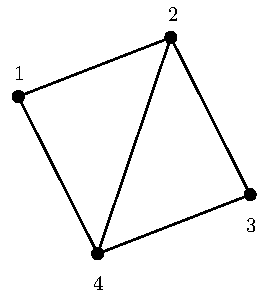
\includegraphics[scale=0.75]{./figuras/pdf/subgrafo0_a.pdf}}
\qquad
\subfloat[]{\label{fig:subgrafo0_b}}{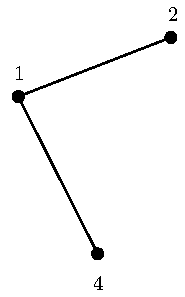
\includegraphics[scale=0.75]{./figuras/pdf/subgrafo0_b.pdf}}
\qquad
\subfloat[]{\label{fig:subgrafo0_c}}{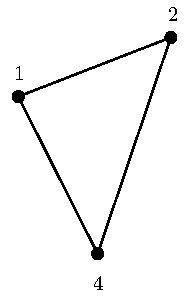
\includegraphics[scale=0.75]{./figuras/pdf/subgrafo0_c.pdf}}
\caption{En \subref{fig:subgrafo0_a} se muestra $G = (V,E)$ donde
$\abs{G} = 4$. Al tomar $V' = \left \lbrace {1,2,4} \right
\rbrace$ se obtiene el subgrafo $H = (V',  \left \lbrace {12,14}
\right \rbrace )$ de \subref{fig:subgrafo0_b}. Finalmente en \subref{fig:subgrafo0_c} se muestra $G[V']$. Claramente $H\subseteq G$ pero $H \neq G[V']$.}
\label{fig:subgrafo0}
\end{figure}

Si $U$ es un conjunto de vértices de $G$, se escribe $G-U$ para
denotar al subgrafo inducido $G[V \setminus U]$. La operación
$G - U$ se denota como \textbf{borrado} de vértices de $G$. En
el caso $G - V(G')$ se escribe $G - G'$. Para $F \subseteq
\binom{V}{2}$ se escribe $G - F \coloneq (V , E \setminus F)$ y
$G + F \coloneq (V, E \cup F)$. En el caso de operar sobre
singletons, tanto para aristas como para vértices, se escribe
$G \pm x$ en vez de $G \pm \lbrace x \rbrace $. La siguiente
proposición permite relacionar las cantidades $\varepsilon(G)$ y
$\varepsilon(H)$ para dos grafos $H \subseteq G$.

\begin{proposition}
	Todo grafo $G$ con al menos una arista, tiene un subgrafo $H$ con
	$\delta(H) > \varepsilon(H) \geq \varepsilon(G)$.
\end{proposition}

\begin{proof}

Se construye una sucesión  $G = G _ { 0 } \supseteq G _ { 1 } \supseteq
\ldots$ de subgrafos inducidos por $G$. En esta sucesión, si el grafo
$i$ - ésimo , $G_i$ tiene un vértice $v_i$ de grado $ d_{G_i}(v_i) \leq
\varepsilon(G_i) $ se genera $G _ { i + 1 } \coloneq G _ { i } - v _ {
i }$. En caso contrario, se termina la sucesión y se define $H \coloneq
G _ { i }$.

Por la elección de $v_i$ se tiene que $\varepsilon \left( G _ { i + 1 }
\right) \geqslant \varepsilon \left( G _ { i } \right)$. Esto se
observa directamente de la relación,
\begin{equation*}
	\frac{|E(G_i)|}{|V(G_i)|} = \frac{|E(G_i)| - \varepsilon(G_i)}{
	|V(G_i)|-1}
\end{equation*}

para todo $i$ en la sucesión. Por construcción, se tendrá entonces
$\varepsilon ( H ) \geqslant \varepsilon ( G )$.

Por otra parte, se observa que $K^{1}$ (grafo consistente de un
vértice), cumple $\varepsilon \left( K ^ { 1 } \right) = 0 <
\varepsilon (G)$. Según la relación anterior, se tendrá entonces que
$K^{1}$ no pertenece a la sucesión, por lo que en particular $H
\neq \emptyset$. Como $H$ es minimal en el sentido de la construcción
(no se pueden borrar más vértices), se tendrá que $\delta ( H ) >
\varepsilon ( H )$.

\end{proof}


Dados dos grafos $G = (V,E)$ y $G' =  (V', E')$ disjuntos, se
denota $G * G'$ como su \textit{join}, al grafo $G * G' \coloneq G
\cup G' + \left \lbrace {xy : x \in V, y \in V' } \right \rbrace$
es decir, $G * G'$ es el grafo resultante al unir $G$ con $G'$,
agregando las aristas resultantes al conectar cada vértice de $G$
con cada vértice de $G'$.

Por otra parte, para dos grafos $G = (V,E)$ y $G' =  (V', E')$
disjuntos, se define el \textbf{producto cartesiano} o simplemente
\textbf{producto} entre grafos $G \ \square \ G'$ como el grafo
cuyo conjunto de aristas es $V(G \ \square \ G')  \coloneq \left (
{ V\times V'} \right ) $. Donde las aristas $u=(u_1,u_2)$ y
$v=(v_1,v_2)$ serán adyacentes, si $u_1 = v_1$ y $u_2 \in
N_{G'}(v_2)$ o $u_2 = v_2$ y $u_1 \in N_{G'}(v_1)$. La figura
(\ref{fig:ej}) muestra el join y el producto de dos
grafos.

\begin{figure}[ht]
\subfloat[]{\label{fig:ej0}}{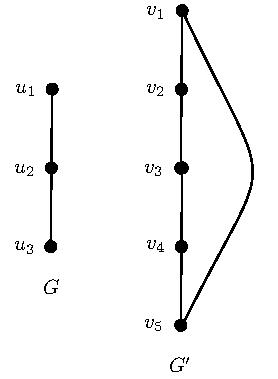
\includegraphics[scale=0.75]{./figuras/pdf/ej.pdf}}
\qquad
\subfloat[]{\label{fig:join}}{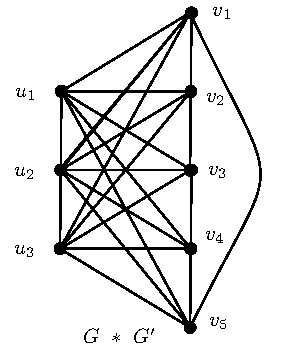
\includegraphics[scale=0.75]{./figuras/pdf/join.pdf}}
\qquad
\subfloat[]{\label{fig:grilla}}{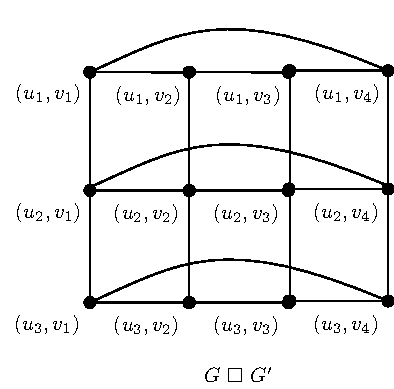
\includegraphics[scale=0.75]{./figuras/pdf/grilla.pdf}}
\caption{En \subref{fig:ej0} se muestran los grafos disjuntos $G$ y $G'$.
El resultado de $G * G'$ se observa en \subref{fig:join}.
Finalmente en \subref{fig:grilla} se muestra $G \ \square \ G'$.}
\label{fig:ej}
\end{figure}


Dados dos grafos $G$ y $H$, es posible definir la noción de
\textbf{morfismo} o transformación entre ambos.

\begin{definition}[morfismo]
\label{def:morfismo}
Dados dos grafos $ G $ y $ H $, un \textbf{morfismo} $f$ de
$ G $ a $ H $ se define como una función $ f : V(G) \rightarrow V(H) $,
que verifica $\forall \  uv \in E(G) \implies f(u)f(v) \in E(H)$.
\end{definition}

\begin{ex}[morfismos entre caminos]
	Se define el grafo $ P_n = ( V, E) $ según la estructura secuencial
	$ V = \left \lbrace {v_0 , \ldots , v_n} \right \rbrace $ donde $ v_i
	\neq v_j, \ \forall i \neq j $. Se tiene además $e_i = v_{i}v_{i+1}$
	para $ E = \left \lbrace {e_0, \ldots, e_{n-1}  } \right \rbrace$.
	Los grafos del tipo $ P_n $ se denotan como \textbf{caminos} de largo
	$n$. En el caso $n=0$ se considera $E = \emptyset$.

	\begin{figure}[ht]
		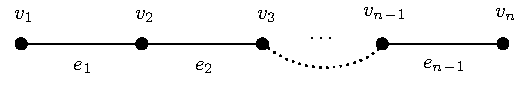
\includegraphics{./figuras/pdf/fig_ex1.pdf}
		\caption{Representación de un camino $P_n$}
		\label{fig:ex1}
	\end{figure}

Estudiar la posibilidad de construir un morfismo entre caminos del tipo
$P_n$ y $P_{n-1}$ para $n \geq 1$.

\end{ex}
\begin{solution}
	Para el caso $n = 1$ no es posible obtener un morfismo, pues $ P_0 $
	no tiene aristas. Para $ n \geq 1 $, se definen los caminos $ P_n $
	con vertices $ V = \left \lbrace {v_0 , \ldots , v_n} \right \rbrace $ y $ P_{n-1} $ con vértices $ V' = \left \lbrace {v_0 , \ldots , v_{n-1} } \right \rbrace $, cada arista de $ P_n $ se denota por $e_i$ para $ i = 0, \ldots, n-1$. De manera análoga (hasta $n-2$) se denotan las aristas de $P_{n-1}$.

	En este caso es posible construir un morfismo $f: V \rightarrow V'$
	a través de :
	\begin{equation*}
		f(v_i) = \begin{cases}
								v_i, \ \ \ \ \ \text{para} \ i=0, \ldots, n-1 \\
								v_{n-2}, \ \text{para} \ i = n
						 \end{cases}
	\end{equation*}

	Por medio de $f$, para cada arista $e_i = v_i v_{i+1} \in E(P_n)$
	existe su arista idéntica $f(v_i)f(v_{i+1}) = e_i \in E(P_{n-1})$ para $i = 1, \ldots, n-2$. Finalmente para la arista $e_{n-1} = v_{n-1} v_{n}$  existe $f(v_{n-1}) (v_{n}) = v_{n-1} v_{n-2} = v_{n-2} v_{n-1} \in E(P_{n-1})$. Por lo que se confirma que $f$ es
	un morfismo entre $P_n$ y $P_{n-1}$.

\end{solution}

\section{Camino y Ciclos}

Un \textbf{camino} es un grafo no vacío $P = (V,E)$  de la forma

\begin{equation*}
	V = \left\{ x _ { 0 } , x _ { 1 } , \ldots , x _ { k } \right\}, \quad
  E = \left\{ x _ { 0 } x _ { 1 } , x _ { 1 } x _ { 2 } , \ldots , x _
	{ k - 1 } x _ { k } \right\}
\end{equation*}

donde los vértices $x_i$ son todos distintos. Los vértices de un camino
se dicen \textit{conectados} por $P$, en particular  $x_0$ y $x_k$ están
conectados por $P$ y se denominan como sus \textit{extremos}. Por otra
parte, los vértices $x _ { 1 } , \dots , x _ { k - 1 }$ son sus
\textit{vértices internos}. El número de aristas en $P$ se denota como
su \textbf{largo}. Un camino de largo $n$ se denota como $P_n$.
